\documentclass[../template]{subfiles}

\begin{document}
\section{Matching}
\subsection{Definizione di Matching}
Dato un grafo non orientato $G = (v, A)$, un matching è un sottoinsieme $M \subseteq A$ dell'insieme di archi $A$ tale che
in $M$ non ci siano coppie di archi adiacenti\footnote{Con un nodo in comune}.
\subsection{Matching a peso massimo}
Di tutti i matching possibili, vogliamo trovare quello il cui peso $w(M) = \sum_{e \in M} w_e$ sia massimo.

\begin{figure}[h]
    \centering
    \begin{tikzpicture}[rotate=90]
        \SetGraphUnit{2}
        \Vertices{circle}{6, 3, 4, 5, 1}
        \WE(6){2}
        \Edge[label=$2$](2)(4)
        \Edge[label=$3$](2)(5)

        \tikzset{EdgeStyle/.style={color=green}}
        \Edge[label=$1$](2)(3)
        \Edge[label=$5$](4)(5)
        \Edge[label=$6$](1)(6)

        \tikzset{EdgeStyle/.style={color=red}}
        \Edge[label=$4$](3)(6)
        \Edge[label=$5$](1)(2)
        ;
    \end{tikzpicture}
\end{figure}

\noindent L'insieme di archi $M_1 = \{ (1, 2) \, (3, 6)\}$ forma un matching di peso $9$, mentre $M_2 = \{(2, 3)\,(4, 5)\,(1, 6)\}$ ha un peso
di $12$.
Algoritmi di matching sono utilizzati per determinare accoppiamenti ottimali tra i nodi.
\\[10pt]
Viene detto matching di \textbf{cardinalità massima}, l'insieme di problemi dove il peso di ogni arco è unitario.
In caso di grafi bipartiti, si cerca una soluzione che colleghi i due set di nodi.
\lstinputlisting[firstline=42, lastline=84]{algorithms/matching.py}

%\subsubsection{Matching iniziale}
%\lstinputlisting{algorithms/initial_match.py}
\subsubsection{Complessità}
$O(\min(|V_1|, |V_2|) |A|)$, quindi polinomiale. Ad ogni iterazione la cardinalità del matching incrementa di 1 unità, appena raggiunta la cardinalità
di $V_1$ e $V_2$ termina. Esiste un algoritmo più efficiente di complessità $O(|V|½|A|)$ ma non è trattato nel corso.

\subsubsection{Note}
Collegando un nodo sorgente alla prima classe di partizione, ed un nodo destinazione alla seconda classe, il problema è riconducibile ad un
problema di flusso massimo, risolvibile con Ford-Fulkerson.

\subsection{Assegnamento}
\end{document}
